\documentclass{article}\usepackage[]{graphicx}\usepackage[]{color}
%% maxwidth is the original width if it is less than linewidth
%% otherwise use linewidth (to make sure the graphics do not exceed the margin)
\makeatletter
\def\maxwidth{ %
  \ifdim\Gin@nat@width>\linewidth
    \linewidth
  \else
    \Gin@nat@width
  \fi
}
\makeatother

\definecolor{fgcolor}{rgb}{0.345, 0.345, 0.345}
\newcommand{\hlnum}[1]{\textcolor[rgb]{0.686,0.059,0.569}{#1}}%
\newcommand{\hlstr}[1]{\textcolor[rgb]{0.192,0.494,0.8}{#1}}%
\newcommand{\hlcom}[1]{\textcolor[rgb]{0.678,0.584,0.686}{\textit{#1}}}%
\newcommand{\hlopt}[1]{\textcolor[rgb]{0,0,0}{#1}}%
\newcommand{\hlstd}[1]{\textcolor[rgb]{0.345,0.345,0.345}{#1}}%
\newcommand{\hlkwa}[1]{\textcolor[rgb]{0.161,0.373,0.58}{\textbf{#1}}}%
\newcommand{\hlkwb}[1]{\textcolor[rgb]{0.69,0.353,0.396}{#1}}%
\newcommand{\hlkwc}[1]{\textcolor[rgb]{0.333,0.667,0.333}{#1}}%
\newcommand{\hlkwd}[1]{\textcolor[rgb]{0.737,0.353,0.396}{\textbf{#1}}}%

\usepackage{framed}
\makeatletter
\newenvironment{kframe}{%
 \def\at@end@of@kframe{}%
 \ifinner\ifhmode%
  \def\at@end@of@kframe{\end{minipage}}%
  \begin{minipage}{\columnwidth}%
 \fi\fi%
 \def\FrameCommand##1{\hskip\@totalleftmargin \hskip-\fboxsep
 \colorbox{shadecolor}{##1}\hskip-\fboxsep
     % There is no \\@totalrightmargin, so:
     \hskip-\linewidth \hskip-\@totalleftmargin \hskip\columnwidth}%
 \MakeFramed {\advance\hsize-\width
   \@totalleftmargin\z@ \linewidth\hsize
   \@setminipage}}%
 {\par\unskip\endMakeFramed%
 \at@end@of@kframe}
\makeatother

\definecolor{shadecolor}{rgb}{.97, .97, .97}
\definecolor{messagecolor}{rgb}{0, 0, 0}
\definecolor{warningcolor}{rgb}{1, 0, 1}
\definecolor{errorcolor}{rgb}{1, 0, 0}
\newenvironment{knitrout}{}{} % an empty environment to be redefined in TeX

\usepackage{alltt}
\IfFileExists{upquote.sty}{\usepackage{upquote}}{}
\begin{document}



\begin{knitrout}
\definecolor{shadecolor}{rgb}{0.969, 0.969, 0.969}\color{fgcolor}\begin{kframe}
\begin{alltt}
\hlcom{## Load libraries}
\hlkwd{library}\hlstd{(splines)}
\hlkwd{library}\hlstd{(MASS)}

\hlcom{## Define the number of tests}
\hlstd{ntest} \hlkwb{<-} \hlnum{1000}

\hlcom{## Set the value of lambda}
\hlstd{lambda} \hlkwb{<-} \hlnum{0.8}

\hlcom{## Set nuber of simulations}
\hlstd{nSims} \hlkwb{<-} \hlnum{10000}
\end{alltt}
\end{kframe}
\end{knitrout}

\section{Probability of being a false positive as a linear function of time}

\begin{knitrout}
\definecolor{shadecolor}{rgb}{0.969, 0.969, 0.969}\color{fgcolor}\begin{kframe}
\begin{alltt}
\hlkwd{set.seed}\hlstd{(}\hlnum{1345}\hlstd{)}

\hlcom{## Set up the time vector and the probability of being null}
\hlstd{tme} \hlkwb{<-} \hlkwd{seq}\hlstd{(}\hlopt{-}\hlnum{1}\hlstd{,}\hlnum{2}\hlstd{,}\hlkwc{length}\hlstd{=ntest)}
\hlstd{pi0} \hlkwb{<-} \hlnum{1}\hlopt{/}\hlnum{4}\hlopt{*}\hlstd{tme}\hlopt{+}\hlnum{1}\hlopt{/}\hlnum{2}

\hlstd{tmeInt} \hlkwb{<-} \hlkwd{cbind}\hlstd{(}\hlnum{1}\hlstd{, tme)}

\hlcom{##save the value of pi0hat for each simulation}
\hlstd{pi0hatMat} \hlkwb{<-} \hlkwd{matrix}\hlstd{(}\hlnum{NA}\hlstd{,} \hlkwc{nrow}\hlstd{=nSims,} \hlkwc{ncol}\hlstd{=ntest)}

\hlkwa{for}\hlstd{(sim} \hlkwa{in} \hlnum{1}\hlopt{:}\hlstd{nSims)}
  \hlstd{\{}
  \hlcom{## Calculate a random variable indicating whether to draw}
  \hlcom{## the p-values from the null or alternative}
  \hlstd{nullI} \hlkwb{<-} \hlkwd{rbinom}\hlstd{(ntest,}\hlkwc{prob}\hlstd{=pi0,}\hlkwc{size}\hlstd{=}\hlnum{1}\hlstd{)}\hlopt{>} \hlnum{0}

  \hlcom{## Sample the null P-values from U(0,1) and the alternatives}
  \hlcom{## from a beta distribution}

  \hlstd{pValues} \hlkwb{<-} \hlkwd{rep}\hlstd{(}\hlnum{NA}\hlstd{,ntest)}
  \hlstd{pValues[nullI]} \hlkwb{<-} \hlkwd{runif}\hlstd{(}\hlkwd{sum}\hlstd{(nullI))}
  \hlstd{pValues[}\hlopt{!}\hlstd{nullI]} \hlkwb{<-} \hlkwd{rbeta}\hlstd{(}\hlkwd{sum}\hlstd{(}\hlopt{!}\hlstd{nullI),}\hlnum{1}\hlstd{,}\hlnum{50}\hlstd{)}

  \hlcom{## Get the estimate}

  \hlstd{y} \hlkwb{<-} \hlstd{pValues} \hlopt{>} \hlstd{lambda}

  \hlstd{glm1} \hlkwb{<-} \hlkwd{lsfit}\hlstd{(tme, y)}

  \hlcom{## Get the estimated pi0 values}
  \hlstd{pi0hatMat[sim, ]} \hlkwb{<-}
    \hlstd{(tmeInt} \hlopt
       \hlkwd{matrix}\hlstd{(glm1}\hlopt{$}\hlstd{coefficients,} \hlkwc{ncol}\hlstd{=}\hlnum{1}\hlstd{))[,}\hlnum{1}\hlstd{]}\hlopt{/}\hlstd{(}\hlnum{1}\hlopt{-}\hlstd{lambda)}
\hlstd{\}}

\hlcom{## Get the mean values:}
\hlstd{pi0hatMean} \hlkwb{<-} \hlkwd{colMeans}\hlstd{(pi0hatMat)}

\hlcom{##Get the variances:}
\hlstd{pi0hatVar} \hlkwb{<-} \hlkwd{apply}\hlstd{(pi0hatMat,} \hlnum{2}\hlstd{, var)}

\hlcom{##Get the variance bounds:}
\hlstd{zMat} \hlkwb{<-} \hlstd{tmeInt}
\hlstd{S} \hlkwb{<-} \hlstd{zMat}\hlopt\hlkwd{solve}\hlstd{(}\hlkwd{t}\hlstd{(zMat)}\hlopt\hlstd{zMat)}\hlopt\hlkwd{t}\hlstd{(zMat)}
\hlstd{pi0hatVarBound} \hlkwb{<-}
  \hlkwd{diag}\hlstd{(S)}\hlopt{/}\hlstd{(}\hlnum{4}\hlopt{*}\hlstd{(}\hlnum{1}\hlopt{-}\hlstd{lambda)}\hlopt{^}\hlnum{2}\hlstd{)}
\end{alltt}
\end{kframe}
\end{knitrout}

\subsection{Plot for means}

\begin{knitrout}
\definecolor{shadecolor}{rgb}{0.969, 0.969, 0.969}\color{fgcolor}\begin{kframe}
\begin{alltt}
\hlkwd{par}\hlstd{(}\hlkwc{cex.axis} \hlstd{=} \hlnum{1.1}\hlstd{,} \hlkwc{cex.main}\hlstd{=}\hlnum{1.3}\hlstd{)}

\hlkwd{plot}\hlstd{(pi0} \hlopt{~} \hlstd{tme,}\hlkwc{col}\hlstd{=}\hlstr{"black"}\hlstd{,}\hlkwc{type}\hlstd{=}\hlstr{"l"}\hlstd{,}\hlkwc{lwd}\hlstd{=}\hlnum{8}\hlstd{,} \hlkwc{lty}\hlstd{=}\hlnum{1}\hlstd{,}
     \hlkwc{xlab}\hlstd{=}\hlstr{""}\hlstd{,} \hlkwc{yaxt} \hlstd{=} \hlstr{"n"}\hlstd{,}
     \hlkwc{ylim}\hlstd{=}\hlkwd{c}\hlstd{(}\hlnum{0}\hlstd{,}\hlnum{1}\hlstd{),} \hlkwc{ylab}\hlstd{=}\hlstr{""}\hlstd{)}
\hlkwd{mtext}\hlstd{(}\hlkwd{expression}\hlstd{(x[i]),} \hlnum{1}\hlstd{,} \hlkwc{line}\hlstd{=}\hlnum{3}\hlstd{,} \hlkwc{cex}\hlstd{=}\hlnum{1.3}\hlstd{)}
\hlkwd{mtext}\hlstd{(}\hlkwd{expression}\hlstd{(}\hlkwd{paste}\hlstd{(}\hlstr{"Mean "}\hlstd{,} \hlkwd{hat}\hlstd{(pi)[}\hlnum{0}\hlstd{](x[i]),}\hlstr{" and "}\hlstd{, pi[}\hlnum{0}\hlstd{](x[i]))),} \hlnum{2}\hlstd{,} \hlkwc{line}\hlstd{=}\hlnum{2}\hlstd{,} \hlkwc{cex}\hlstd{=}\hlnum{1.3}\hlstd{)}
\hlkwd{points}\hlstd{(pi0hatMean} \hlopt{~} \hlstd{tme,}\hlkwc{col}\hlstd{=}\hlstr{"orange"}\hlstd{,}\hlkwc{type}\hlstd{=}\hlstr{"l"}\hlstd{,}\hlkwc{lwd}\hlstd{=}\hlnum{3}\hlstd{,} \hlkwc{lty}\hlstd{=}\hlnum{2}\hlstd{)}
\hlkwd{legend}\hlstd{(}\hlkwc{x}\hlstd{=}\hlopt{-}\hlnum{0.4}\hlstd{,} \hlkwc{y}\hlstd{=}\hlnum{0.2}\hlstd{,}
       \hlkwc{legend}\hlstd{=}\hlkwd{c}\hlstd{(}\hlstr{"Truth"}\hlstd{,} \hlstr{"Simple linear regression"}\hlstd{),}
       \hlkwc{col}\hlstd{=}\hlkwd{c}\hlstd{(}\hlstr{"black"}\hlstd{,} \hlstr{"orange"}\hlstd{),} \hlkwc{bty}\hlstd{=}\hlstr{"n"}\hlstd{,}
       \hlkwc{lwd}\hlstd{=}\hlkwd{c}\hlstd{(}\hlnum{8}\hlstd{,}\hlnum{3}\hlstd{),} \hlkwc{lty}\hlstd{=}\hlkwd{c}\hlstd{(}\hlnum{1}\hlstd{,}\hlnum{2}\hlstd{),}
       \hlkwc{cex}\hlstd{=}\hlnum{1.2}\hlstd{,} \hlkwc{x.intersp}\hlstd{=}\hlnum{0.2}\hlstd{,} \hlkwc{y.intersp}\hlstd{=}\hlnum{1.0}\hlstd{)}
\hlkwd{axis}\hlstd{(}\hlkwc{side}\hlstd{=}\hlnum{2}\hlstd{,} \hlkwc{at}\hlstd{=(}\hlnum{0}\hlopt{:}\hlnum{5}\hlstd{)}\hlopt{/}\hlnum{5}\hlstd{,} \hlkwc{mgp}\hlstd{=}\hlkwd{c}\hlstd{(}\hlnum{3}\hlstd{,} \hlnum{0.7}\hlstd{,} \hlnum{0}\hlstd{))}
\end{alltt}
\end{kframe}

{\centering 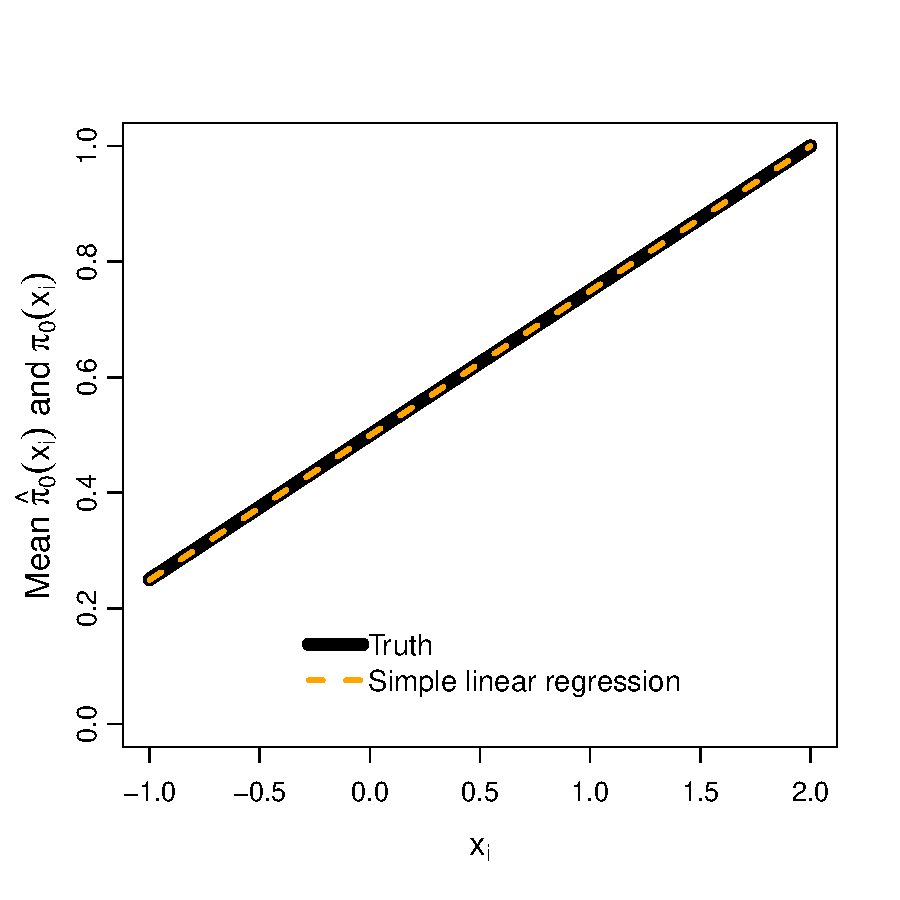
\includegraphics[width=\maxwidth]{figures/Fig1a-1} 

}



\end{knitrout}

\subsection{Plot for variances}

\begin{knitrout}
\definecolor{shadecolor}{rgb}{0.969, 0.969, 0.969}\color{fgcolor}\begin{kframe}
\begin{alltt}
\hlkwd{par}\hlstd{(}\hlkwc{cex.axis} \hlstd{=} \hlnum{1.1}\hlstd{,} \hlkwc{cex.main}\hlstd{=}\hlnum{1.3}\hlstd{)}

\hlkwd{plot}\hlstd{(pi0hatVarBound} \hlopt{~} \hlstd{tme,} \hlkwc{col}\hlstd{=}\hlstr{"red"}\hlstd{,} \hlkwc{ylim}\hlstd{=}\hlkwd{c}\hlstd{(}\hlnum{0}\hlstd{,} \hlkwd{max}\hlstd{(pi0hatVarBound)),}
     \hlkwc{lwd}\hlstd{=}\hlnum{3}\hlstd{,} \hlkwc{lty}\hlstd{=}\hlnum{3}\hlstd{,}
     \hlkwc{type}\hlstd{=}\hlstr{"l"}\hlstd{,}
     \hlkwc{xlab}\hlstd{=}\hlstr{""}\hlstd{,} \hlkwc{ylab}\hlstd{=}\hlstr{""}\hlstd{)}
\hlkwd{mtext}\hlstd{(}\hlkwd{expression}\hlstd{(x[i]),} \hlnum{1}\hlstd{,} \hlkwc{line}\hlstd{=}\hlnum{3}\hlstd{,} \hlkwc{cex}\hlstd{=}\hlnum{1.3}\hlstd{)}
\hlkwd{mtext}\hlstd{(}\hlkwd{expression}\hlstd{(}\hlkwd{paste}\hlstd{(}\hlstr{"Variance and upper bound of variance for "}\hlstd{,} \hlstr{" "}\hlstd{,} \hlkwd{hat}\hlstd{(pi)[}\hlnum{0}\hlstd{](x[i]),} \hlkwc{sep}\hlstd{=}\hlstr{" "}\hlstd{)),} \hlnum{2}\hlstd{,} \hlkwc{line}\hlstd{=}\hlnum{2}\hlstd{,} \hlkwc{cex}\hlstd{=}\hlnum{1.3}\hlstd{)}
\hlkwd{points}\hlstd{(pi0hatVar} \hlopt{~} \hlstd{tme,} \hlkwc{col}\hlstd{=}\hlstr{"black"}\hlstd{,} \hlkwc{type}\hlstd{=}\hlstr{"l"}\hlstd{,} \hlkwc{lwd}\hlstd{=}\hlnum{3}\hlstd{,} \hlkwc{lty}\hlstd{=}\hlnum{1}\hlstd{)}
\hlkwd{legend}\hlstd{(}\hlstr{"top"}\hlstd{,} \hlcom{##x=-0.4, y=0.2, }
       \hlkwc{legend}\hlstd{=}\hlkwd{c}\hlstd{(}\hlstr{"Empirical variance"}\hlstd{,} \hlstr{"Upper bound"}\hlstd{),}
       \hlkwc{col}\hlstd{=}\hlkwd{c}\hlstd{(}\hlstr{"black"}\hlstd{,} \hlstr{"red"}\hlstd{),} \hlkwc{bty}\hlstd{=}\hlstr{"n"}\hlstd{,}
       \hlkwc{lwd}\hlstd{=}\hlkwd{c}\hlstd{(}\hlnum{3}\hlstd{,}\hlnum{3}\hlstd{),} \hlkwc{lty}\hlstd{=}\hlkwd{c}\hlstd{(}\hlnum{1}\hlstd{,}\hlnum{3}\hlstd{),}
       \hlkwc{cex}\hlstd{=}\hlnum{1.2}\hlstd{,} \hlkwc{x.intersp}\hlstd{=}\hlnum{0.2}\hlstd{,} \hlkwc{y.intersp}\hlstd{=}\hlnum{1.0}\hlstd{)}
\end{alltt}
\end{kframe}

{\centering 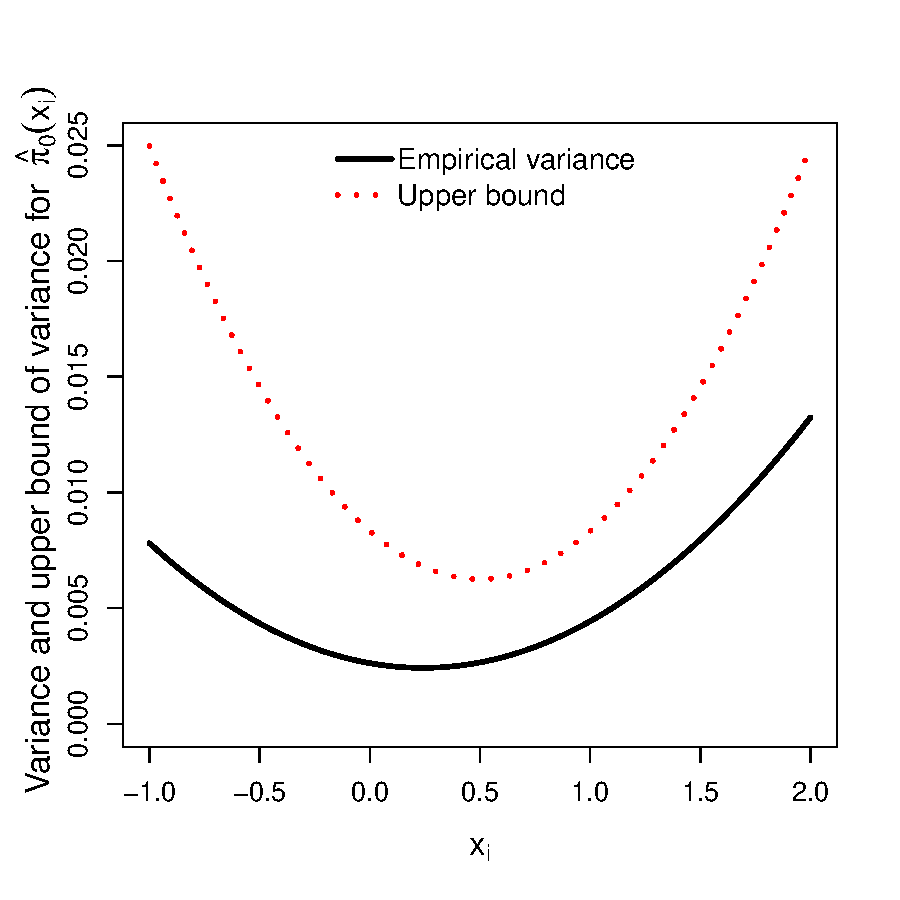
\includegraphics[width=\maxwidth]{figures/Fig2a-1} 

}



\end{knitrout}

\section{Probability of being a false positive as a smooth function of time}

\begin{knitrout}
\definecolor{shadecolor}{rgb}{0.969, 0.969, 0.969}\color{fgcolor}\begin{kframe}
\begin{alltt}
\hlkwd{set.seed}\hlstd{(}\hlnum{1345}\hlstd{)}

\hlcom{## Set up the time vector and the probability of being null}
\hlstd{tme} \hlkwb{<-} \hlkwd{seq}\hlstd{(}\hlopt{-}\hlnum{1}\hlstd{,}\hlnum{2}\hlstd{,}\hlkwc{length}\hlstd{=ntest)}
\hlstd{pi0} \hlkwb{<-} \hlkwd{pnorm}\hlstd{(tme)}

\hlcom{##save the value of pi0hat for each simulation}
\hlcom{##fitting splines:}
\hlstd{pi0hatMatFitSpl} \hlkwb{<-} \hlkwd{matrix}\hlstd{(}\hlnum{NA}\hlstd{,} \hlkwc{nrow}\hlstd{=nSims,} \hlkwc{ncol}\hlstd{=ntest)}
\hlcom{##fitting linear function:}
\hlstd{pi0hatMatFitLin} \hlkwb{<-} \hlstd{pi0hatMatFitSpl}

\hlstd{splineMat} \hlkwb{<-} \hlkwd{ns}\hlstd{(tme,}\hlkwc{df}\hlstd{=}\hlnum{3}\hlstd{)}
\hlstd{splineMatInt} \hlkwb{<-} \hlkwd{cbind}\hlstd{(}\hlnum{1}\hlstd{, splineMat)}

\hlkwa{for}\hlstd{(sim} \hlkwa{in} \hlnum{1}\hlopt{:}\hlstd{nSims)}
  \hlstd{\{}
  \hlcom{## Calculate a random variable indicating whether to draw}
  \hlcom{## the p-values from the null or alternative}
  \hlstd{nullI} \hlkwb{<-} \hlkwd{rbinom}\hlstd{(ntest,}\hlkwc{prob}\hlstd{=pi0,}\hlkwc{size}\hlstd{=}\hlnum{1}\hlstd{)}\hlopt{>} \hlnum{0}

  \hlcom{## Sample the null P-values from U(0,1) and the alternatives}
  \hlcom{## from a beta distribution}

  \hlstd{pValues} \hlkwb{<-} \hlkwd{rep}\hlstd{(}\hlnum{NA}\hlstd{,ntest)}
  \hlstd{pValues[nullI]} \hlkwb{<-} \hlkwd{runif}\hlstd{(}\hlkwd{sum}\hlstd{(nullI))}
  \hlstd{pValues[}\hlopt{!}\hlstd{nullI]} \hlkwb{<-} \hlkwd{rbeta}\hlstd{(}\hlkwd{sum}\hlstd{(}\hlopt{!}\hlstd{nullI),}\hlnum{1}\hlstd{,}\hlnum{50}\hlstd{)}

  \hlcom{## Get the estimates}

  \hlstd{y} \hlkwb{<-} \hlstd{pValues} \hlopt{>} \hlstd{lambda}

  \hlstd{glm1} \hlkwb{<-} \hlkwd{lsfit}\hlstd{(splineMat, y)}
  \hlcom{## Get the estimated pi0 values  }
  \hlstd{pi0hatMatFitSpl[sim, ]} \hlkwb{<-}
    \hlstd{(splineMatInt} \hlopt
       \hlkwd{matrix}\hlstd{(glm1}\hlopt{$}\hlstd{coefficients,} \hlkwc{ncol}\hlstd{=}\hlnum{1}\hlstd{))[,}\hlnum{1}\hlstd{]}\hlopt{/}\hlstd{(}\hlnum{1}\hlopt{-}\hlstd{lambda)}

  \hlstd{glm2} \hlkwb{<-} \hlkwd{lsfit}\hlstd{(tme, y)}
  \hlcom{## Get the estimated pi0 values  }
  \hlstd{pi0hatMatFitLin[sim, ]} \hlkwb{<-}
    \hlstd{(}\hlkwd{cbind}\hlstd{(}\hlnum{1}\hlstd{, tme)} \hlopt
       \hlkwd{matrix}\hlstd{(glm2}\hlopt{$}\hlstd{coefficients,} \hlkwc{ncol}\hlstd{=}\hlnum{1}\hlstd{))[,}\hlnum{1}\hlstd{]}\hlopt{/}\hlstd{(}\hlnum{1}\hlopt{-}\hlstd{lambda)}
\hlstd{\}}

\hlcom{## Get the mean values:}
\hlstd{pi0hatMeanFitSpl} \hlkwb{<-} \hlkwd{colMeans}\hlstd{(pi0hatMatFitSpl)}
\hlstd{pi0hatMeanFitLin} \hlkwb{<-} \hlkwd{colMeans}\hlstd{(pi0hatMatFitLin)}

\hlcom{##Get the variances:}
\hlstd{pi0hatVarFitSpl} \hlkwb{<-} \hlkwd{apply}\hlstd{(pi0hatMatFitSpl,} \hlnum{2}\hlstd{, var)}
\hlstd{pi0hatVarFitLin} \hlkwb{<-} \hlkwd{apply}\hlstd{(pi0hatMatFitLin,} \hlnum{2}\hlstd{, var)}

\hlcom{##Get the variance bounds:}
\hlstd{zMat} \hlkwb{<-} \hlstd{splineMatInt}
\hlstd{S} \hlkwb{<-} \hlstd{zMat}\hlopt\hlkwd{solve}\hlstd{(}\hlkwd{t}\hlstd{(zMat)}\hlopt\hlstd{zMat)}\hlopt\hlkwd{t}\hlstd{(zMat)}
\hlstd{pi0hatVarBoundFitSpl} \hlkwb{<-}
  \hlkwd{diag}\hlstd{(S)}\hlopt{/}\hlstd{(}\hlnum{4}\hlopt{*}\hlstd{(}\hlnum{1}\hlopt{-}\hlstd{lambda)}\hlopt{^}\hlnum{2}\hlstd{)}

\hlstd{zMat} \hlkwb{<-} \hlkwd{cbind}\hlstd{(}\hlnum{1}\hlstd{, tme)}
\hlstd{S} \hlkwb{<-} \hlstd{zMat}\hlopt\hlkwd{solve}\hlstd{(}\hlkwd{t}\hlstd{(zMat)}\hlopt\hlstd{zMat)}\hlopt\hlkwd{t}\hlstd{(zMat)}
\hlstd{pi0hatVarBoundFitLin} \hlkwb{<-}
  \hlkwd{diag}\hlstd{(S)}\hlopt{/}\hlstd{(}\hlnum{4}\hlopt{*}\hlstd{(}\hlnum{1}\hlopt{-}\hlstd{lambda)}\hlopt{^}\hlnum{2}\hlstd{)}
\end{alltt}
\end{kframe}
\end{knitrout}

\subsection{Plot for means}

\begin{knitrout}
\definecolor{shadecolor}{rgb}{0.969, 0.969, 0.969}\color{fgcolor}\begin{kframe}
\begin{alltt}
\hlkwd{par}\hlstd{(}\hlkwc{cex.axis} \hlstd{=} \hlnum{1.1}\hlstd{,} \hlkwc{cex.main}\hlstd{=}\hlnum{1.3}\hlstd{)}

\hlkwd{plot}\hlstd{(pi0} \hlopt{~} \hlstd{tme,}\hlkwc{col}\hlstd{=}\hlstr{"black"}\hlstd{,}\hlkwc{type}\hlstd{=}\hlstr{"l"}\hlstd{,}\hlkwc{lwd}\hlstd{=}\hlnum{8}\hlstd{,} \hlkwc{lty}\hlstd{=}\hlnum{1}\hlstd{,}
     \hlkwc{xlab}\hlstd{=}\hlstr{""}\hlstd{,} \hlkwc{yaxt} \hlstd{=} \hlstr{"n"}\hlstd{,}
     \hlkwc{ylim}\hlstd{=}\hlkwd{c}\hlstd{(}\hlnum{0}\hlstd{,}\hlnum{1}\hlstd{),} \hlkwc{ylab}\hlstd{=}\hlstr{""}\hlstd{)}
\hlkwd{mtext}\hlstd{(}\hlkwd{expression}\hlstd{(x[i]),} \hlnum{1}\hlstd{,} \hlkwc{line}\hlstd{=}\hlnum{3}\hlstd{,} \hlkwc{cex}\hlstd{=}\hlnum{1.3}\hlstd{)}
\hlkwd{mtext}\hlstd{(}\hlkwd{expression}\hlstd{(}\hlkwd{paste}\hlstd{(}\hlstr{"Mean "}\hlstd{,} \hlkwd{hat}\hlstd{(pi)[}\hlnum{0}\hlstd{](x[i]),}\hlstr{" and "}\hlstd{, pi[}\hlnum{0}\hlstd{](x[i]))),} \hlnum{2}\hlstd{,} \hlkwc{line}\hlstd{=}\hlnum{2}\hlstd{,} \hlkwc{cex}\hlstd{=}\hlnum{1.3}\hlstd{)}
\hlkwd{points}\hlstd{(pi0hatMeanFitSpl} \hlopt{~} \hlstd{tme,}
       \hlkwc{col}\hlstd{=}\hlstr{"orange"}\hlstd{,}\hlkwc{type}\hlstd{=}\hlstr{"l"}\hlstd{,}\hlkwc{lwd}\hlstd{=}\hlnum{3}\hlstd{,} \hlkwc{lty}\hlstd{=}\hlnum{2}\hlstd{)}
\hlkwd{points}\hlstd{(pi0hatMeanFitLin} \hlopt{~} \hlstd{tme,}
       \hlkwc{col}\hlstd{=}\hlstr{"blue"}\hlstd{,}\hlkwc{type}\hlstd{=}\hlstr{"l"}\hlstd{,}\hlkwc{lwd}\hlstd{=}\hlnum{3}\hlstd{,} \hlkwc{lty}\hlstd{=}\hlnum{4}\hlstd{)}
\hlkwd{legend}\hlstd{(}\hlstr{"bottomright"}\hlstd{,} \hlcom{##x=-100, y=0.3, }
       \hlkwc{legend}\hlstd{=}\hlkwd{c}\hlstd{(}\hlstr{"Truth"}\hlstd{,} \hlstr{"B-splines with\textbackslash{}n3 degrees of freedom"}\hlstd{,} \hlstr{"Simple linear regression"}\hlstd{),}
       \hlkwc{col}\hlstd{=}\hlkwd{c}\hlstd{(}\hlstr{"black"}\hlstd{,} \hlstr{"orange"}\hlstd{,} \hlstr{"blue"}\hlstd{),} \hlkwc{bty}\hlstd{=}\hlstr{"n"}\hlstd{,}
       \hlkwc{lwd}\hlstd{=}\hlkwd{c}\hlstd{(}\hlnum{8}\hlstd{,}\hlnum{3}\hlstd{,}\hlnum{3}\hlstd{),} \hlkwc{lty}\hlstd{=}\hlkwd{c}\hlstd{(}\hlnum{1}\hlstd{,}\hlnum{2}\hlstd{,}\hlnum{4}\hlstd{),}
       \hlkwc{cex}\hlstd{=}\hlnum{1.2}\hlstd{,} \hlkwc{x.intersp}\hlstd{=}\hlnum{0.2}\hlstd{,} \hlkwc{y.intersp}\hlstd{=}\hlnum{1.0}\hlstd{)}
\hlkwd{axis}\hlstd{(}\hlkwc{side}\hlstd{=}\hlnum{2}\hlstd{,} \hlkwc{at}\hlstd{=(}\hlnum{0}\hlopt{:}\hlnum{5}\hlstd{)}\hlopt{/}\hlnum{5}\hlstd{,} \hlkwc{mgp}\hlstd{=}\hlkwd{c}\hlstd{(}\hlnum{3}\hlstd{,} \hlnum{0.7}\hlstd{,} \hlnum{0}\hlstd{))}
\end{alltt}
\end{kframe}

{\centering 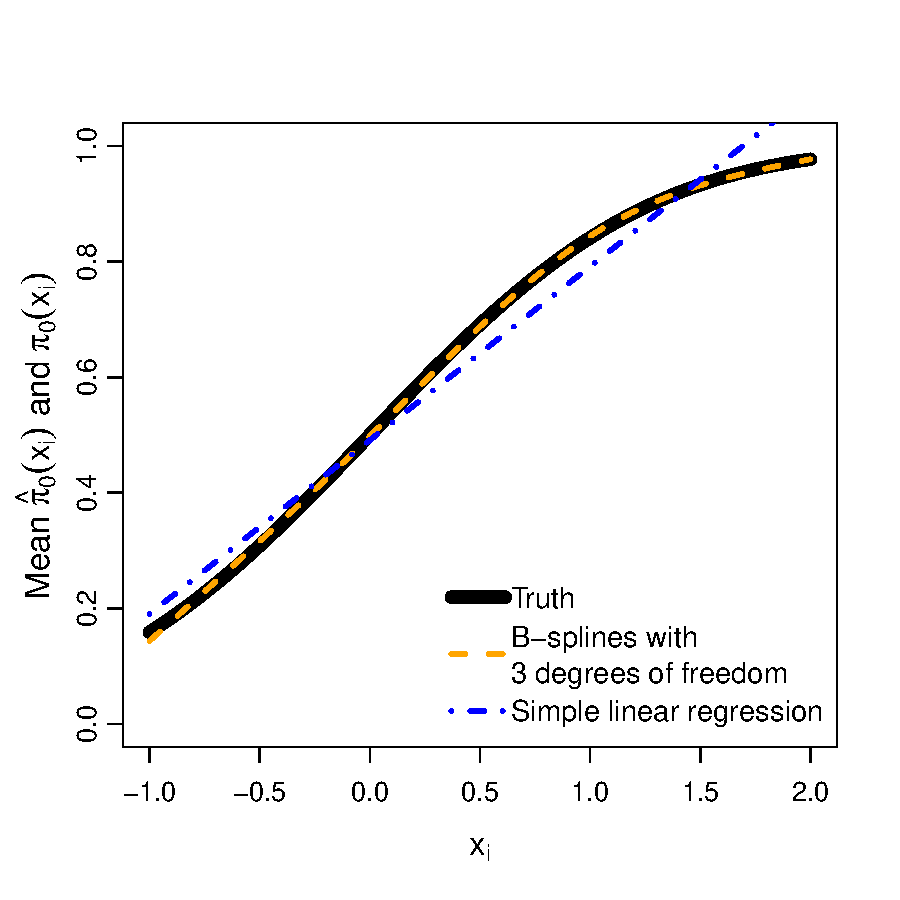
\includegraphics[width=\maxwidth]{figures/Fig1b-1} 

}



\end{knitrout}

\subsection{Plots for variances}

\begin{knitrout}
\definecolor{shadecolor}{rgb}{0.969, 0.969, 0.969}\color{fgcolor}\begin{kframe}
\begin{alltt}
\hlkwd{par}\hlstd{(}\hlkwc{cex.axis} \hlstd{=} \hlnum{1.1}\hlstd{,} \hlkwc{cex.main}\hlstd{=}\hlnum{1.3}\hlstd{)}

\hlkwd{plot}\hlstd{(pi0hatVarBoundFitLin} \hlopt{~} \hlstd{tme,} \hlkwc{col}\hlstd{=}\hlstr{"red"}\hlstd{,} \hlkwc{ylim}\hlstd{=}\hlkwd{c}\hlstd{(}\hlnum{0}\hlstd{,} \hlkwd{max}\hlstd{(pi0hatVarBoundFitLin)),}
     \hlkwc{lwd}\hlstd{=}\hlnum{3}\hlstd{,} \hlkwc{lty}\hlstd{=}\hlnum{3}\hlstd{,}
     \hlkwc{type}\hlstd{=}\hlstr{"l"}\hlstd{,}
     \hlkwc{xlab}\hlstd{=}\hlstr{""}\hlstd{,} \hlkwc{ylab}\hlstd{=}\hlstr{""}\hlstd{)}
\hlkwd{mtext}\hlstd{(}\hlkwd{expression}\hlstd{(x[i]),} \hlnum{1}\hlstd{,} \hlkwc{line}\hlstd{=}\hlnum{3}\hlstd{,} \hlkwc{cex}\hlstd{=}\hlnum{1.3}\hlstd{)}
\hlkwd{mtext}\hlstd{(}\hlkwd{expression}\hlstd{(}\hlkwd{paste}\hlstd{(}\hlstr{"Variance and upper bound of variance for "}\hlstd{,} \hlstr{" "}\hlstd{,} \hlkwd{hat}\hlstd{(pi)[}\hlnum{0}\hlstd{](x[i]),} \hlkwc{sep}\hlstd{=}\hlstr{" "}\hlstd{)),} \hlnum{2}\hlstd{,} \hlkwc{line}\hlstd{=}\hlnum{2}\hlstd{,} \hlkwc{cex}\hlstd{=}\hlnum{1.3}\hlstd{)}
\hlkwd{points}\hlstd{(pi0hatVarFitLin} \hlopt{~} \hlstd{tme,} \hlkwc{col}\hlstd{=}\hlstr{"black"}\hlstd{,} \hlkwc{type}\hlstd{=}\hlstr{"l"}\hlstd{,} \hlkwc{lwd}\hlstd{=}\hlnum{3}\hlstd{,} \hlkwc{lty}\hlstd{=}\hlnum{1}\hlstd{)}
\hlkwd{legend}\hlstd{(}\hlstr{"top"}\hlstd{,} \hlcom{##x=-0.4, y=0.2, }
       \hlkwc{legend}\hlstd{=}\hlkwd{c}\hlstd{(}\hlstr{"Empirical variance"}\hlstd{,} \hlstr{"Upper bound"}\hlstd{),}
       \hlkwc{col}\hlstd{=}\hlkwd{c}\hlstd{(}\hlstr{"black"}\hlstd{,} \hlstr{"red"}\hlstd{),} \hlkwc{bty}\hlstd{=}\hlstr{"n"}\hlstd{,}
       \hlkwc{lwd}\hlstd{=}\hlkwd{c}\hlstd{(}\hlnum{3}\hlstd{,}\hlnum{3}\hlstd{),} \hlkwc{lty}\hlstd{=}\hlkwd{c}\hlstd{(}\hlnum{1}\hlstd{,}\hlnum{3}\hlstd{),}
       \hlkwc{cex}\hlstd{=}\hlnum{1.2}\hlstd{,} \hlkwc{x.intersp}\hlstd{=}\hlnum{0.2}\hlstd{,} \hlkwc{y.intersp}\hlstd{=}\hlnum{1.0}\hlstd{)}
\end{alltt}
\end{kframe}

{\centering 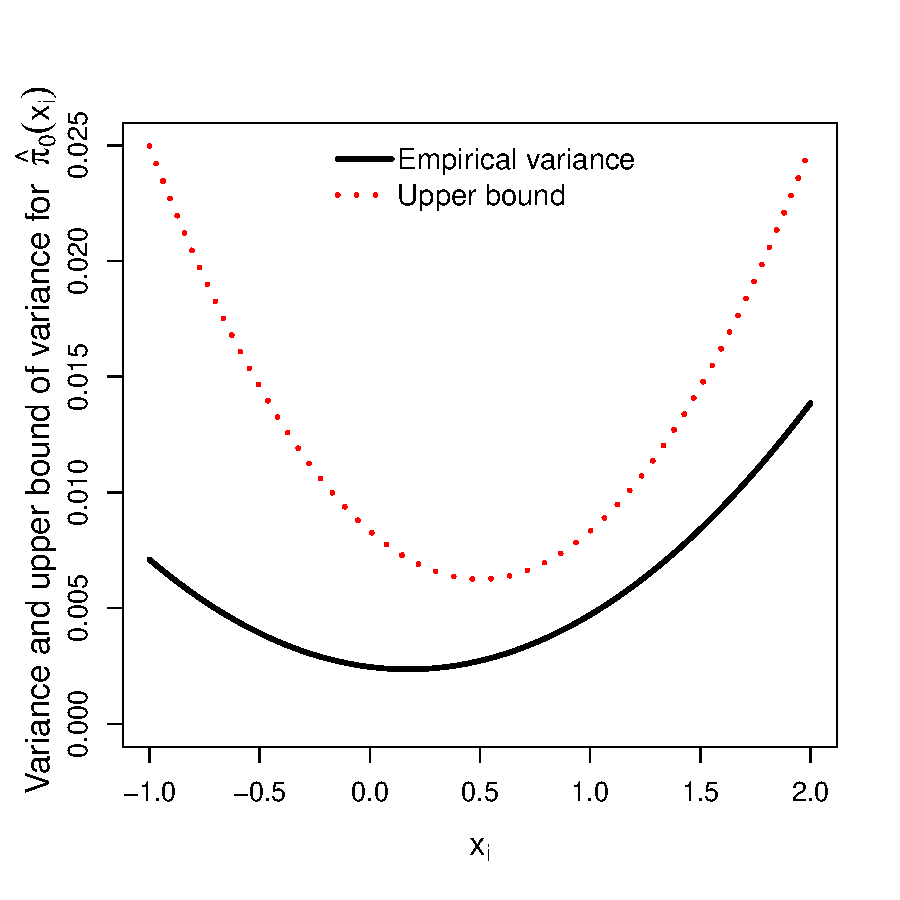
\includegraphics[width=\maxwidth]{figures/Fig2b-1} 

}



\end{knitrout}

\begin{knitrout}
\definecolor{shadecolor}{rgb}{0.969, 0.969, 0.969}\color{fgcolor}\begin{kframe}
\begin{alltt}
\hlkwd{par}\hlstd{(}\hlkwc{cex.axis} \hlstd{=} \hlnum{1.1}\hlstd{,} \hlkwc{cex.main}\hlstd{=}\hlnum{1.3}\hlstd{)}

\hlkwd{plot}\hlstd{(pi0hatVarBoundFitSpl} \hlopt{~} \hlstd{tme,} \hlkwc{col}\hlstd{=}\hlstr{"red"}\hlstd{,} \hlkwc{ylim}\hlstd{=}\hlkwd{c}\hlstd{(}\hlnum{0}\hlstd{,} \hlkwd{max}\hlstd{(pi0hatVarBoundFitSpl)),}
     \hlkwc{lwd}\hlstd{=}\hlnum{3}\hlstd{,} \hlkwc{lty}\hlstd{=}\hlnum{3}\hlstd{,}
     \hlkwc{type}\hlstd{=}\hlstr{"l"}\hlstd{,}
     \hlkwc{xlab}\hlstd{=}\hlstr{""}\hlstd{,} \hlkwc{ylab}\hlstd{=}\hlstr{""}\hlstd{)}
\hlkwd{mtext}\hlstd{(}\hlkwd{expression}\hlstd{(x[i]),} \hlnum{1}\hlstd{,} \hlkwc{line}\hlstd{=}\hlnum{3}\hlstd{,} \hlkwc{cex}\hlstd{=}\hlnum{1.3}\hlstd{)}
\hlkwd{mtext}\hlstd{(}\hlkwd{expression}\hlstd{(}\hlkwd{paste}\hlstd{(}\hlstr{"Variance and upper bound of variance for "}\hlstd{,} \hlstr{" "}\hlstd{,} \hlkwd{hat}\hlstd{(pi)[}\hlnum{0}\hlstd{](x[i]),} \hlkwc{sep}\hlstd{=}\hlstr{" "}\hlstd{)),} \hlnum{2}\hlstd{,} \hlkwc{line}\hlstd{=}\hlnum{2}\hlstd{,} \hlkwc{cex}\hlstd{=}\hlnum{1.3}\hlstd{)}
\hlkwd{points}\hlstd{(pi0hatVarFitSpl} \hlopt{~} \hlstd{tme,} \hlkwc{col}\hlstd{=}\hlstr{"black"}\hlstd{,} \hlkwc{type}\hlstd{=}\hlstr{"l"}\hlstd{,} \hlkwc{lwd}\hlstd{=}\hlnum{3}\hlstd{,} \hlkwc{lty}\hlstd{=}\hlnum{1}\hlstd{)}
\hlkwd{legend}\hlstd{(}\hlstr{"top"}\hlstd{,} \hlcom{##x=-0.4, y=0.2, }
       \hlkwc{legend}\hlstd{=}\hlkwd{c}\hlstd{(}\hlstr{"Empirical variance"}\hlstd{,} \hlstr{"Upper bound"}\hlstd{),}
       \hlkwc{col}\hlstd{=}\hlkwd{c}\hlstd{(}\hlstr{"black"}\hlstd{,} \hlstr{"red"}\hlstd{),} \hlkwc{bty}\hlstd{=}\hlstr{"n"}\hlstd{,}
       \hlkwc{lwd}\hlstd{=}\hlkwd{c}\hlstd{(}\hlnum{3}\hlstd{,}\hlnum{3}\hlstd{),} \hlkwc{lty}\hlstd{=}\hlkwd{c}\hlstd{(}\hlnum{1}\hlstd{,}\hlnum{3}\hlstd{),}
       \hlkwc{cex}\hlstd{=}\hlnum{1.2}\hlstd{,} \hlkwc{x.intersp}\hlstd{=}\hlnum{0.2}\hlstd{,} \hlkwc{y.intersp}\hlstd{=}\hlnum{1.0}\hlstd{)}
\end{alltt}
\end{kframe}

{\centering 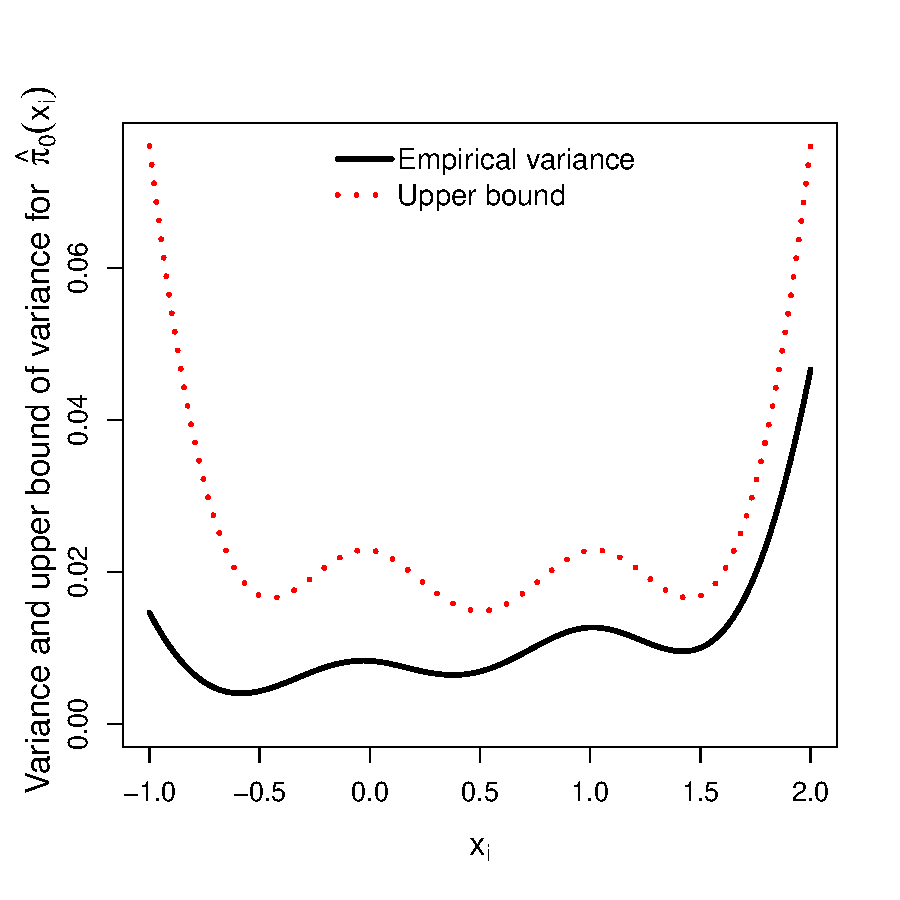
\includegraphics[width=\maxwidth]{figures/Fig2c-1} 

}



\end{knitrout}

\section{Probability of being a false positive as a sine + step function}

\begin{knitrout}
\definecolor{shadecolor}{rgb}{0.969, 0.969, 0.969}\color{fgcolor}\begin{kframe}
\begin{alltt}
\hlkwd{set.seed}\hlstd{(}\hlnum{1345}\hlstd{)}

\hlcom{## Set up the time vector and the probability of being null}
\hlstd{tme1} \hlkwb{<-} \hlkwd{seq}\hlstd{(}\hlopt{-}\hlnum{1}\hlopt{*}\hlstd{pi,}\hlnum{2}\hlopt{*}\hlstd{pi,}\hlkwc{length}\hlstd{=ntest)}
\hlstd{tme2} \hlkwb{<-} \hlkwd{rep}\hlstd{(}\hlnum{1}\hlopt{:}\hlnum{0}\hlstd{,} \hlkwc{each}\hlstd{=ntest}\hlopt{/}\hlnum{2}\hlstd{)}
\hlstd{pi0} \hlkwb{<-} \hlnum{1}\hlopt{/}\hlnum{4}\hlopt{*}\hlkwd{sin}\hlstd{(tme1)} \hlopt{+} \hlstd{tme2}\hlopt{/}\hlnum{4} \hlopt{+} \hlnum{1}\hlopt{/}\hlnum{2}
\hlcom{##pi0 <- 1/4*sin(tme1) + 0.5}
\hlkwd{range}\hlstd{(pi0)}
\end{alltt}
\begin{verbatim}
## [1] 0.2500028 0.9999972
\end{verbatim}
\begin{alltt}
\hlstd{splineMat3} \hlkwb{<-} \hlkwd{cbind}\hlstd{(}\hlkwd{ns}\hlstd{(tme1,}\hlkwc{df}\hlstd{=}\hlnum{3}\hlstd{), tme2)}
\hlstd{splineMat20} \hlkwb{<-} \hlkwd{cbind}\hlstd{(}\hlkwd{ns}\hlstd{(tme1,}\hlkwc{df}\hlstd{=}\hlnum{20}\hlstd{), tme2)}
\hlstd{splineMatInt3} \hlkwb{<-} \hlkwd{cbind}\hlstd{(}\hlnum{1}\hlstd{, splineMat3)}
\hlstd{splineMatInt20} \hlkwb{<-} \hlkwd{cbind}\hlstd{(}\hlnum{1}\hlstd{, splineMat20)}

\hlcom{##save the value of pi0hat for each simulation}
\hlstd{pi0hatMat3} \hlkwb{<-} \hlstd{pi0hatMat20} \hlkwb{<-}
  \hlkwd{matrix}\hlstd{(}\hlnum{NA}\hlstd{,} \hlkwc{nrow}\hlstd{=nSims,} \hlkwc{ncol}\hlstd{=ntest)}

\hlkwa{for}\hlstd{(sim} \hlkwa{in} \hlnum{1}\hlopt{:}\hlstd{nSims)}
\hlstd{\{}
  \hlcom{## Calculate a random variable indicating whether to draw}
  \hlcom{## the p-values from the null or alternative}
  \hlstd{nullI} \hlkwb{<-} \hlkwd{rbinom}\hlstd{(ntest,}\hlkwc{prob}\hlstd{=pi0,}\hlkwc{size}\hlstd{=}\hlnum{1}\hlstd{)}\hlopt{>} \hlnum{0}

  \hlcom{## Sample the null P-values from U(0,1) and the alternatives}
  \hlcom{## from a beta distribution}

  \hlstd{pValues} \hlkwb{<-} \hlkwd{rep}\hlstd{(}\hlnum{NA}\hlstd{,ntest)}
  \hlstd{pValues[nullI]} \hlkwb{<-} \hlkwd{runif}\hlstd{(}\hlkwd{sum}\hlstd{(nullI))}
  \hlstd{pValues[}\hlopt{!}\hlstd{nullI]} \hlkwb{<-} \hlkwd{rbeta}\hlstd{(}\hlkwd{sum}\hlstd{(}\hlopt{!}\hlstd{nullI),}\hlnum{1}\hlstd{,}\hlnum{50}\hlstd{)}

  \hlcom{## Get the estimate}

  \hlstd{y} \hlkwb{<-} \hlstd{pValues} \hlopt{>} \hlstd{lambda}

  \hlstd{glm1} \hlkwb{<-} \hlkwd{lsfit}\hlstd{(splineMat3, y)}
  \hlcom{## Get the estimate pi0 values}
  \hlstd{pi0hatMat3[sim, ]} \hlkwb{<-} \hlstd{(splineMatInt3} \hlopt
                          \hlkwd{matrix}\hlstd{(glm1}\hlopt{$}\hlstd{coefficients,}
                                 \hlkwc{ncol}\hlstd{=}\hlnum{1}\hlstd{))[,}\hlnum{1}\hlstd{]}\hlopt{/}\hlstd{(}\hlnum{1}\hlopt{-}\hlstd{lambda)}

  \hlstd{glm2} \hlkwb{<-} \hlkwd{lsfit}\hlstd{(splineMat20, y)}
  \hlcom{## Get the estimate pi0 values}
  \hlstd{pi0hatMat20[sim, ]} \hlkwb{<-} \hlstd{(splineMatInt20} \hlopt
                           \hlkwd{matrix}\hlstd{(glm2}\hlopt{$}\hlstd{coefficients,}
                                  \hlkwc{ncol}\hlstd{=}\hlnum{1}\hlstd{))[,}\hlnum{1}\hlstd{]}\hlopt{/}\hlstd{(}\hlnum{1}\hlopt{-}\hlstd{lambda)}
\hlstd{\}}

\hlcom{## Get the mean values:}
\hlstd{pi0hatMean3} \hlkwb{<-} \hlkwd{colMeans}\hlstd{(pi0hatMat3)}
\hlstd{pi0hatMean20} \hlkwb{<-} \hlkwd{colMeans}\hlstd{(pi0hatMat20)}

\hlcom{##Get the variances:}
\hlstd{pi0hatVar3} \hlkwb{<-} \hlkwd{apply}\hlstd{(pi0hatMat3,} \hlnum{2}\hlstd{, var)}
\hlstd{pi0hatVar20} \hlkwb{<-} \hlkwd{apply}\hlstd{(pi0hatMat20,} \hlnum{2}\hlstd{, var)}

\hlcom{##Get the variance bounds:}
\hlstd{zMat} \hlkwb{<-} \hlstd{splineMatInt3}
\hlstd{S} \hlkwb{<-} \hlstd{zMat}\hlopt\hlkwd{ginv}\hlstd{(}\hlkwd{t}\hlstd{(zMat)}\hlopt\hlstd{zMat)}\hlopt\hlkwd{t}\hlstd{(zMat)}
\hlstd{pi0hatVarBound3} \hlkwb{<-}
  \hlkwd{diag}\hlstd{(S)}\hlopt{/}\hlstd{(}\hlnum{4}\hlopt{*}\hlstd{(}\hlnum{1}\hlopt{-}\hlstd{lambda)}\hlopt{^}\hlnum{2}\hlstd{)}

\hlstd{zMat} \hlkwb{<-} \hlstd{splineMatInt20}
\hlstd{S} \hlkwb{<-} \hlstd{zMat}\hlopt\hlkwd{ginv}\hlstd{(}\hlkwd{t}\hlstd{(zMat)}\hlopt\hlstd{zMat)}\hlopt\hlkwd{t}\hlstd{(zMat)}
\hlstd{pi0hatVarBound20} \hlkwb{<-}
  \hlkwd{diag}\hlstd{(S)}\hlopt{/}\hlstd{(}\hlnum{4}\hlopt{*}\hlstd{(}\hlnum{1}\hlopt{-}\hlstd{lambda)}\hlopt{^}\hlnum{2}\hlstd{)}
\end{alltt}
\end{kframe}
\end{knitrout}

\subsection{Plot for means}

\begin{knitrout}
\definecolor{shadecolor}{rgb}{0.969, 0.969, 0.969}\color{fgcolor}\begin{kframe}
\begin{alltt}
\hlkwd{par}\hlstd{(}\hlkwc{cex.axis} \hlstd{=} \hlnum{1.1}\hlstd{,} \hlkwc{cex.main}\hlstd{=}\hlnum{1.3}\hlstd{)}

\hlkwd{plot}\hlstd{(pi0} \hlopt{~} \hlstd{tme1,}\hlkwc{col}\hlstd{=}\hlstr{"black"}\hlstd{,}\hlkwc{type}\hlstd{=}\hlstr{"l"}\hlstd{,}\hlkwc{lwd}\hlstd{=}\hlnum{8}\hlstd{,} \hlkwc{lty}\hlstd{=}\hlnum{1}\hlstd{,}
     \hlkwc{xlab}\hlstd{=}\hlstr{""}\hlstd{,} \hlkwc{yaxt} \hlstd{=} \hlstr{"n"}\hlstd{,}
     \hlkwc{ylim}\hlstd{=}\hlkwd{c}\hlstd{(}\hlnum{0}\hlstd{,}\hlnum{1}\hlstd{),} \hlkwc{ylab}\hlstd{=}\hlstr{""}\hlstd{)}
\hlkwd{mtext}\hlstd{(}\hlkwd{expression}\hlstd{(x[i1]),} \hlnum{1}\hlstd{,} \hlkwc{line}\hlstd{=}\hlnum{3}\hlstd{,} \hlkwc{cex}\hlstd{=}\hlnum{1.3}\hlstd{)}
\hlkwd{mtext}\hlstd{(}\hlkwd{expression}\hlstd{(}\hlkwd{paste}\hlstd{(}\hlstr{"Mean "}\hlstd{,} \hlkwd{hat}\hlstd{(pi)[}\hlnum{0}\hlstd{](x[i]),}\hlstr{" and "}\hlstd{,}
                       \hlstd{pi[}\hlnum{0}\hlstd{](x[i]))),} \hlnum{2}\hlstd{,} \hlkwc{line}\hlstd{=}\hlnum{2}\hlstd{,} \hlkwc{cex}\hlstd{=}\hlnum{1.3}\hlstd{)}
\hlkwd{points}\hlstd{(pi0hatMean20} \hlopt{~} \hlstd{tme1,}\hlkwc{col}\hlstd{=}\hlstr{"orange"}\hlstd{,}\hlkwc{type}\hlstd{=}\hlstr{"l"}\hlstd{,}\hlkwc{lwd}\hlstd{=}\hlnum{3}\hlstd{,} \hlkwc{lty}\hlstd{=}\hlnum{2}\hlstd{)}
\hlkwd{points}\hlstd{(pi0hatMean3} \hlopt{~} \hlstd{tme1,}\hlkwc{col}\hlstd{=}\hlstr{"blue"}\hlstd{,}\hlkwc{type}\hlstd{=}\hlstr{"l"}\hlstd{,}\hlkwc{lwd}\hlstd{=}\hlnum{3}\hlstd{,} \hlkwc{lty}\hlstd{=}\hlnum{4}\hlstd{)}

\hlkwd{legend}\hlstd{(}\hlstr{"bottomright"}\hlstd{,} \hlcom{##x=-100, y=0.3, }
       \hlkwc{legend}\hlstd{=}\hlkwd{c}\hlstd{(}\hlstr{"Truth"}\hlstd{,} \hlstr{"B-splines with\textbackslash{}n20 degrees of freedom"}\hlstd{,}
                \hlstr{"B-splines with\textbackslash{}n3 degrees of freedom"}\hlstd{),}
       \hlkwc{col}\hlstd{=}\hlkwd{c}\hlstd{(}\hlstr{"black"}\hlstd{,} \hlstr{"orange"}\hlstd{,} \hlstr{"blue"}\hlstd{),} \hlkwc{bty}\hlstd{=}\hlstr{"n"}\hlstd{,}
       \hlkwc{lwd}\hlstd{=}\hlkwd{c}\hlstd{(}\hlnum{8}\hlstd{,}\hlnum{3}\hlstd{,}\hlnum{3}\hlstd{),} \hlkwc{lty}\hlstd{=}\hlkwd{c}\hlstd{(}\hlnum{1}\hlstd{,}\hlnum{2}\hlstd{,}\hlnum{4}\hlstd{),}
       \hlkwc{cex}\hlstd{=}\hlnum{1.2}\hlstd{,} \hlkwc{x.intersp}\hlstd{=}\hlnum{0.2}\hlstd{,} \hlkwc{y.intersp}\hlstd{=}\hlnum{1.15}\hlstd{)}
\hlkwd{axis}\hlstd{(}\hlkwc{side}\hlstd{=}\hlnum{2}\hlstd{,} \hlkwc{at}\hlstd{=(}\hlnum{0}\hlopt{:}\hlnum{5}\hlstd{)}\hlopt{/}\hlnum{5}\hlstd{,} \hlkwc{mgp}\hlstd{=}\hlkwd{c}\hlstd{(}\hlnum{3}\hlstd{,} \hlnum{0.7}\hlstd{,} \hlnum{0}\hlstd{))}
\end{alltt}
\end{kframe}

{\centering 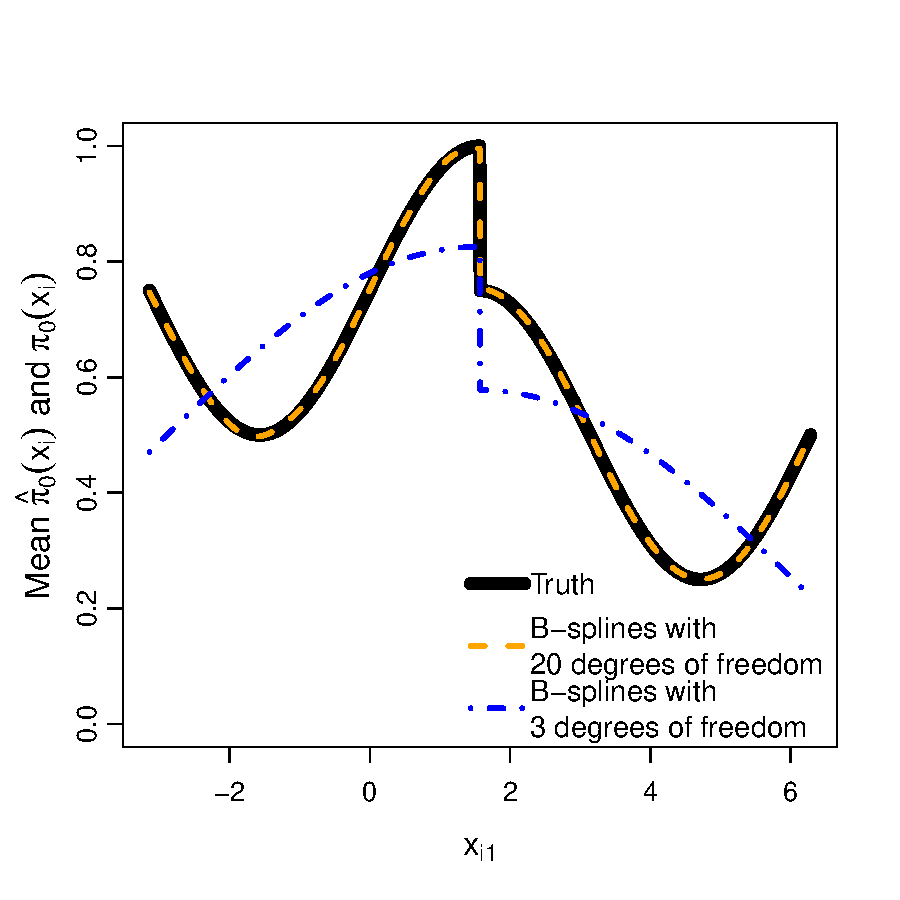
\includegraphics[width=\maxwidth]{figures/Fig1c-1} 

}



\end{knitrout}

\subsection{Plots for variances}

\begin{knitrout}
\definecolor{shadecolor}{rgb}{0.969, 0.969, 0.969}\color{fgcolor}\begin{kframe}
\begin{alltt}
\hlkwd{par}\hlstd{(}\hlkwc{cex.axis} \hlstd{=} \hlnum{1.1}\hlstd{,} \hlkwc{cex.main}\hlstd{=}\hlnum{1.3}\hlstd{)}

\hlkwd{plot}\hlstd{(pi0hatVarBound3} \hlopt{~} \hlstd{tme1,} \hlkwc{col}\hlstd{=}\hlstr{"red"}\hlstd{,} \hlkwc{ylim}\hlstd{=}\hlkwd{c}\hlstd{(}\hlnum{0}\hlstd{,} \hlkwd{max}\hlstd{(pi0hatVarBound3)),}
     \hlkwc{lwd}\hlstd{=}\hlnum{3}\hlstd{,} \hlkwc{lty}\hlstd{=}\hlnum{3}\hlstd{,}
     \hlkwc{type}\hlstd{=}\hlstr{"l"}\hlstd{,}
     \hlkwc{xlab}\hlstd{=}\hlstr{""}\hlstd{,} \hlkwc{ylab}\hlstd{=}\hlstr{""}\hlstd{)}
\hlkwd{mtext}\hlstd{(}\hlkwd{expression}\hlstd{(x[i1]),} \hlnum{1}\hlstd{,} \hlkwc{line}\hlstd{=}\hlnum{3}\hlstd{,} \hlkwc{cex}\hlstd{=}\hlnum{1.3}\hlstd{)}
\hlkwd{mtext}\hlstd{(}\hlkwd{expression}\hlstd{(}\hlkwd{paste}\hlstd{(}\hlstr{"Variance and upper bound of variance for "}\hlstd{,} \hlstr{" "}\hlstd{,} \hlkwd{hat}\hlstd{(pi)[}\hlnum{0}\hlstd{](x[i]),} \hlkwc{sep}\hlstd{=}\hlstr{" "}\hlstd{)),} \hlnum{2}\hlstd{,} \hlkwc{line}\hlstd{=}\hlnum{2}\hlstd{,} \hlkwc{cex}\hlstd{=}\hlnum{1.3}\hlstd{)}
\hlkwd{points}\hlstd{(pi0hatVar3} \hlopt{~} \hlstd{tme1,} \hlkwc{col}\hlstd{=}\hlstr{"black"}\hlstd{,} \hlkwc{type}\hlstd{=}\hlstr{"l"}\hlstd{,} \hlkwc{lwd}\hlstd{=}\hlnum{3}\hlstd{,} \hlkwc{lty}\hlstd{=}\hlnum{1}\hlstd{)}
\hlkwd{legend}\hlstd{(}\hlstr{"top"}\hlstd{,} \hlcom{##x=-0.4, y=0.2, }
       \hlkwc{legend}\hlstd{=}\hlkwd{c}\hlstd{(}\hlstr{"Empirical variance"}\hlstd{,} \hlstr{"Upper bound"}\hlstd{),}
       \hlkwc{col}\hlstd{=}\hlkwd{c}\hlstd{(}\hlstr{"black"}\hlstd{,} \hlstr{"red"}\hlstd{),} \hlkwc{bty}\hlstd{=}\hlstr{"n"}\hlstd{,}
       \hlkwc{lwd}\hlstd{=}\hlkwd{c}\hlstd{(}\hlnum{3}\hlstd{,}\hlnum{3}\hlstd{),} \hlkwc{lty}\hlstd{=}\hlkwd{c}\hlstd{(}\hlnum{1}\hlstd{,}\hlnum{3}\hlstd{),}
       \hlkwc{cex}\hlstd{=}\hlnum{1.2}\hlstd{,} \hlkwc{x.intersp}\hlstd{=}\hlnum{0.2}\hlstd{,} \hlkwc{y.intersp}\hlstd{=}\hlnum{1.0}\hlstd{)}
\end{alltt}
\end{kframe}

{\centering 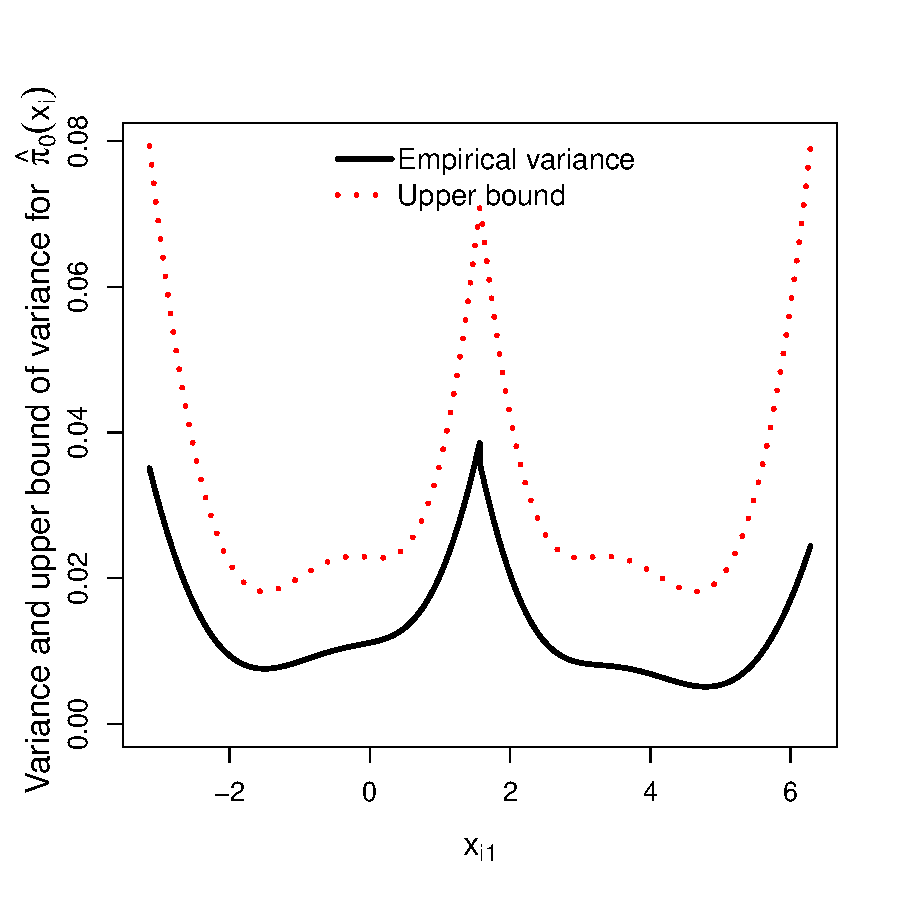
\includegraphics[width=\maxwidth]{figures/Fig2d-1} 

}



\end{knitrout}

\begin{knitrout}
\definecolor{shadecolor}{rgb}{0.969, 0.969, 0.969}\color{fgcolor}\begin{kframe}
\begin{alltt}
\hlkwd{par}\hlstd{(}\hlkwc{cex.axis} \hlstd{=} \hlnum{1.1}\hlstd{,} \hlkwc{cex.main}\hlstd{=}\hlnum{1.3}\hlstd{)}

\hlkwd{plot}\hlstd{(pi0hatVarBound20} \hlopt{~} \hlstd{tme1,} \hlkwc{col}\hlstd{=}\hlstr{"red"}\hlstd{,} \hlkwc{ylim}\hlstd{=}\hlkwd{c}\hlstd{(}\hlnum{0}\hlstd{,} \hlkwd{max}\hlstd{(pi0hatVarBound20)),}
     \hlkwc{lwd}\hlstd{=}\hlnum{3}\hlstd{,} \hlkwc{lty}\hlstd{=}\hlnum{3}\hlstd{,}
     \hlkwc{type}\hlstd{=}\hlstr{"l"}\hlstd{,}
     \hlkwc{xlab}\hlstd{=}\hlstr{""}\hlstd{,} \hlkwc{ylab}\hlstd{=}\hlstr{""}\hlstd{)}
\hlkwd{mtext}\hlstd{(}\hlkwd{expression}\hlstd{(x[i1]),} \hlnum{1}\hlstd{,} \hlkwc{line}\hlstd{=}\hlnum{3}\hlstd{,} \hlkwc{cex}\hlstd{=}\hlnum{1.3}\hlstd{)}
\hlkwd{mtext}\hlstd{(}\hlkwd{expression}\hlstd{(}\hlkwd{paste}\hlstd{(}\hlstr{"Variance and upper bound of variance for "}\hlstd{,} \hlstr{" "}\hlstd{,} \hlkwd{hat}\hlstd{(pi)[}\hlnum{0}\hlstd{](x[i]),} \hlkwc{sep}\hlstd{=}\hlstr{" "}\hlstd{)),} \hlnum{2}\hlstd{,} \hlkwc{line}\hlstd{=}\hlnum{2}\hlstd{,} \hlkwc{cex}\hlstd{=}\hlnum{1.3}\hlstd{)}
\hlkwd{points}\hlstd{(pi0hatVar20} \hlopt{~} \hlstd{tme1,} \hlkwc{col}\hlstd{=}\hlstr{"black"}\hlstd{,} \hlkwc{type}\hlstd{=}\hlstr{"l"}\hlstd{,} \hlkwc{lwd}\hlstd{=}\hlnum{3}\hlstd{,} \hlkwc{lty}\hlstd{=}\hlnum{1}\hlstd{)}
\hlkwd{legend}\hlstd{(}\hlstr{"top"}\hlstd{,} \hlcom{##x=-0.4, y=0.2, }
       \hlkwc{legend}\hlstd{=}\hlkwd{c}\hlstd{(}\hlstr{"Empirical variance"}\hlstd{,} \hlstr{"Upper bound"}\hlstd{),}
       \hlkwc{col}\hlstd{=}\hlkwd{c}\hlstd{(}\hlstr{"black"}\hlstd{,} \hlstr{"red"}\hlstd{),} \hlkwc{bty}\hlstd{=}\hlstr{"n"}\hlstd{,}
       \hlkwc{lwd}\hlstd{=}\hlkwd{c}\hlstd{(}\hlnum{3}\hlstd{,}\hlnum{3}\hlstd{),} \hlkwc{lty}\hlstd{=}\hlkwd{c}\hlstd{(}\hlnum{1}\hlstd{,}\hlnum{3}\hlstd{),}
       \hlkwc{cex}\hlstd{=}\hlnum{1.2}\hlstd{,} \hlkwc{x.intersp}\hlstd{=}\hlnum{0.2}\hlstd{,} \hlkwc{y.intersp}\hlstd{=}\hlnum{1.0}\hlstd{)}
\end{alltt}
\end{kframe}

{\centering 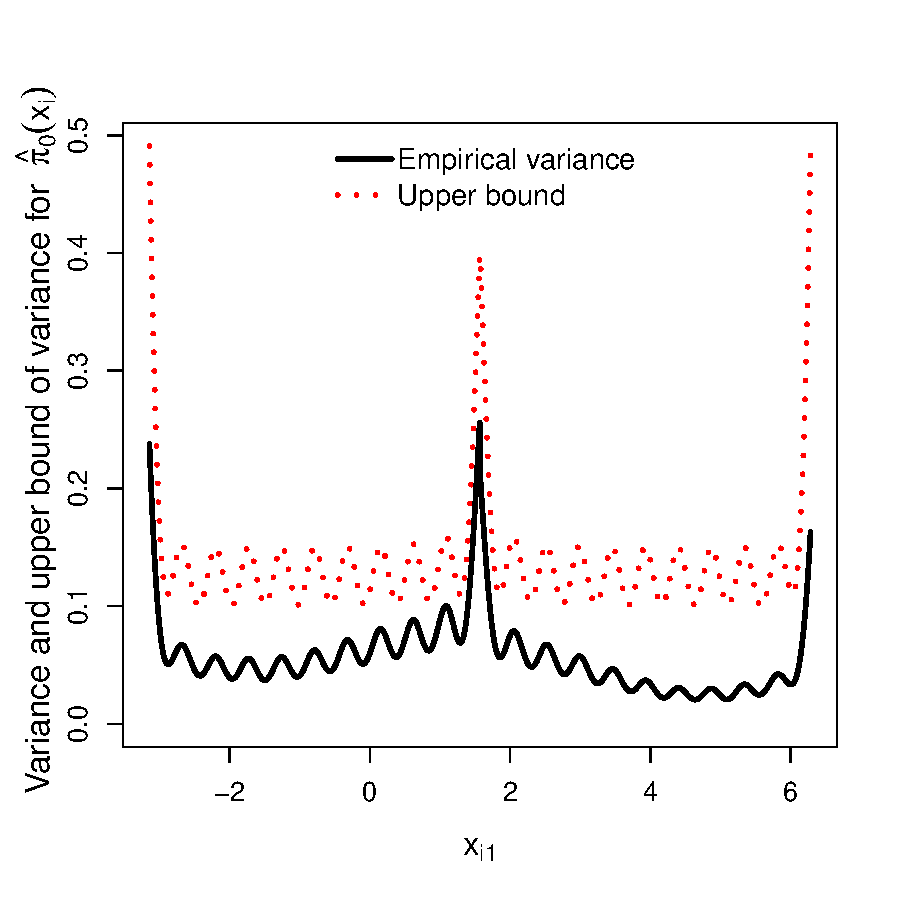
\includegraphics[width=\maxwidth]{figures/Fig2e-1} 

}



\end{knitrout}


\end{document}
